%
% This is Chapter 8 file (chap8.tex)
%
\chapter{Magnetic Field Topology Reconstruction Using Machine Learning Algorithm} \label{chap:chap8}

    \section{Overview} \label{sec:ovrvw8}

        Machine learning\index{Machine Learning}, over the last decade has become increasingly relevant in data and image
        analysis. Both, image reconstruction and data imputation, specifically in a time series,
        have increasingly relied on machine learning techniques and algorithm \citep{Wang2018,
        Bertsimas2017}. In this chapter we apply one such algorithm/technique to a synthetically
        generated time series dataset of the magnetic field derived from a fully kinetic 3-D
        simulation of space plasma. This work serves as a proof of concept for a future mission
        consisting of multiple spacecraft that would map out the topology of the solar-wind's
        magnetic field.

        \Cref{sec:intr8} motivates the multi-spacecraft observation of space plasmas and the
        reconstruction of 3-D magnetic field structure. \Cref{sec:bgnd8} presents the current state
        of the field. Synthetic data generation is discussed in \Cref{sec:data8} and
        \Cref{sec:meth8} discusses the methodology used in detail. \Cref{sec:diss8} presents the
        results of the implemented algorithm. The conclusion of the study is summarized in
        \Cref{sec:conc8} along with some discussion and suggestions of future works\footnote{Part of
        this study was published in \citet{Maruca2021}.}.

    \section{Introduction} \label{sec:intr8}

        Over the last 7 decades in-situ observation of solar wind has been carried by different
        spacecraft starting with Sputnik in 1957 and on going with the most recent mission Solar
        Orbiter which was launched in 2020. Majority of such missions launched a single spacecraft.
        Observations from these missions have vastly improved and enhanced our understanding of
        solar wind and its dynamics, thanks to ever increasing, more precise and detailed
        observations. However, single spacecraft missions cannot differentiate between a temporal
        and spatial fluctuation. This also means we do not have detailed information of the full 3-D
        structure of the interplanetary magnetic field. To address this, a few missions have flown
        with 4 or 5 spacecraft (e.g.,
        \discolorlinks{\href{http://www.esa.int/Science_Exploration/Space_Science/Cluster_overview2}{Cluster}},
        \discolorlinks{\href{https://www.nasa.gov/themis-and-artemis}{THEMIS-ARTEMIS}}, and
        \discolorlinks{\href{https://www.nasa.gov/mission_pages/mms/overview/index.html}{MMS}}), and
        missions with even more spacecraft have been proposed \citep{Klein2019a}. Though work done
        by \citet{Fu2015} and \citet{Torbert2020} using MMS data are promising, they are limited to
        a single scale. Methodology employed by \citet{Fu2015} also becomes inaccurate if the
        distance between spacecraft is of the order of ion-inertial length ($d_{\rm i}$). Given the
        multi-scale nature of solar wind \citep{Verscharen2019} we must have a system where we can
        study the magnetic field by reconstructing it at multiple scales. So far no mission has
        succeeded in generating a full three dimensional image of the magnetic vector field in the
        solar wind, mostly because of large number of spacecraft required to carry out such a task
        and at various length scales. A full 3-D image would provide magnetic field vector at every
        point within the area being imaged and thus will be able to trace the interplanetary
        magnetic field lines. It will also get us information related to structure and topology,
        which are extremely important for understanding turbulence and its evolution in space
        plasmas, especially how energy is stored in and transported through the plasma.

        Though an active field of research, not much work has been done in this from the vantage
        point of machine learning. In this study we present a proof of concept of magnetic field’s
        topology reconstruction using multi-point observation in a 3-D simulation box. For
        multi-point observation, we fly a constellation of virtual spacecraft through a simulation
        box (see \Cref{sec:data8}), and carry out the interpolation on observed vector data in the
        3-D space along its trajectory using Gaussian Processes Regression in machine learning. The
        study also explores the number of spacecraft, the relative separation between them, and
        their configuration required for resolving structures of various scales.

    \section{Background} \label{sec:bgnd8}

        Spacecraft make regular in-situ measurement as plasma convects over them. Reconstructing the
        full 3-D topology of interplanetary magnetic field thus requires interpolating the data from
        the finite set of spacecraft observations. Different interpolation techniques can be used to
        achieve this result. Since solar wind is multi-scale in nature \citep{Verscharen2019} we
        will need sufficiently large number of observations to reliably construct the magnetic field
        at various different scales. For a planar configuration of a constellation of spacecraft
        where normal to the plane of orientation is in parallel (or anti-parallel) to the solar wind
        direction, as employed in this study (see \Cref{sec:data8} and \Cref{fig:spc_conf}), we can
        make more observations in the parallel flow direction by increasing the cadence of measuring
        instrument, whereas in the direction perpendicular to the flow, same effect can be achieved
        by increasing the number of spacecraft.
        
        For interpolation between the observation points, because of the presence of non-linear
        structures (see \Cref{chap:chap5}) and sharp discontinuities (see \Cref{chap:chap6}), linear
        interpolation techniques might not be best suited. We thus turn to machine learning
        algorithms in an effort to minimize the number of spacecraft needed and maximize the
        feasibility of such a space mission. Several such machine learning methods for the purpose
        of data imputation have been explored in literature \citep{Lin2019, Bertsimas2017,
        Wang2018}. As discussed in \citet{Lin2019}, the best solution or the most appropriate method
        depends largely on the domain of the problem. What works for one kind of dataset might
        completely fail for a slightly different one, as we will see in this study as well. For our
        purpose, we decided to explore GP and develop an algorithm based on it. The rest of this
        section gives a brief description of GP, some of its salient features, and its key
        advantages and disadvantages.

        \subsection{Gaussian Processes Regression} \label{sec:gpr}

            Gaussian Processes\index{Machine Learning!Gaussian Processes} (GP) as a generic term means that a dataset with finite number of
            observation is modelled as if it were a multivariate normal distribution
            \citep{Gramacy2020}. It is a probability distribution over possible functions that fit a
            given finite dataset. Just as a Gaussian distribution is fully characterised by its mean
            ($\mu$)~and covariance~($\Sigma$), a GP is completely defined by (1) a mean function
            $m(x)$ indicating the mean at any point of the input space and (2) a covariance function
            $K(x,x')$ that sets the covariance between input pairs \textbf{x} and \textbf{x}$'$
            \citep{Rasmussen2006}. These can be written as:
            \begin{align}
                \begin{split}
                    m(\mathbf{x}) & = \mathbb{E}[f(\mathbf{x})] \\
                    k(\mathbf{x},\mathbf{x}') & = \mathbb{E}[(f(\mathbf{x})- m(\mathbf{x}))(f(\mathbf{x}')- m(\mathbf{x}'))] \label{eq:gpr_mx_kx}
                \end{split}
            \end{align}
            and Gaussian processes can be written as:
            \begin{align}
                 f(\mathbf{x}) & \sim \mathcal{GP}\left(m(\mathbf{x}), k(\mathbf{x}, \mathbf{x}')\right) \label{eq:gpr_gp}
            \end{align}
            The covariance matrices in \Cref{eq:gpr_mx_kx} can be computed using a predefined
            function, which are referred as kernels in GP. This sets a prior to the set of functions
            which must be considered for a given dataset and the type of kernel chosen defines the
            characteristics of this prior.

            There are several standard kernels (see \Cref{sec:meth8}). For this study, we tried a
            few which were available through one the Python packages and selected the one most
            suitable for our dataset.

            One of the advantages of using GP in this application is that it is non-parametric and
            thus, doesn't require a priory fit function to model the input data. It is particularly
            relevant to our case since we do not have much information about the structure of the
            solar wind. Rather than relying on fit function, GP look at every possible model and
            probabilistically explore the space to find the most optimal one for a given dataset.
            Naively, it will appear that there are infinite functions to be considered here since
            the probabilistic approach used in GP considers all possible functions. In reality, this
            is not the case since each function is assigned a prior and the infinite number of
            functions are defined by their statistics, making the whole method a lot more
            manageable. Another advantage of GP is its computational tractability
            \citep{Rasmussen2006}.
            
            Selection of an appropriate kernel, though important to the whole process is not
            critical, as even if we choose a random kernel it often does a decent job of data
            imputation.  Recent development in Deep GP in fact do away with the issue of
            pre-defining a kernel since it is designed to learn the kernel which works best for a
            given dataset \citep{Bui2016}. Well calibrated predictive uncertainty estimates and ease
            of generalization, for both regression and classification analyses, are other benefits
            of using GP.

            As with any method, there are some disadvantages associated with it. One of the major
            drawback of GP is its computational cost. Since inversion of matrices is required, which
            makes the method of $\mathcal{O}(n^3)$, it is computationally very expensive to run for
            large number of data points (n~$>$~2000) \citep{Gramacy2020}.

    \section{Kernels in Gaussian Processes} \label{sec:meth8}

        For this study we implemented GP using
        \discolorlinks{\href{https://scikit-learn.org/stable/index.html}{SciKit Learn}} package
        available in Python \citep{Pedregosa2011}. SciKit has a few default kernels\index{Machine Learning!kernels} implemented in
        the package, we list out some of them here:

        \begin{enumerate}
            \item Constant Kernel (CK)
            \item Radial-basis Function Kernel (RBF)
            \item Mat\'ern Kernel (MK)
            \item Rational Quadratic Kernel (RQ)
            \item Exponential-Sine-Squared Kernel (ESS)
        \end{enumerate}
        For our study we used these five kernels either individually or in combination with each
        other. We briefly discuss each of the aforementioned kernels here. A more in-depth
        discussion of each kernel can be found in \citet{Rasmussen2006} or on the
        \discolorlinks{\href{https://scikit-learn.org/stable/modules/gaussian_process.html\#kernels-for-gaussian-processes}{SciKit
        Learn}}
        web-page\footnote{https://scikit-learn.org/stable/modules/gaussian\_process.html\#kernels-for-gaussian-processes}.\\
        \\
        \textbf{1.\,Constant Kernel\index{Machine Learning!kernels!constant}}: By definition this is simply a constant number or a vector for
        all points in the space. This is largely useful in combination with other kernels where
        either modification of magnitude (Product kernel) or change of mean (Sum kernel) is
        required. The kernel can be written as:
        \begin{align}
            \begin{split}
                k(x_{\rm i},x_{\rm j}) & = constant\_value \;\forall\; x_{\rm i}, x_{\rm j} \label{eq:cst_ker}
            \end{split}
        \end{align}
        \\
        \textbf{2.\,Radial-basis Function kernel\index{Machine Learning!kernels!RBF}}: The RBF kernel is also known as ``squared
        exponential kernel". The kernel has one length parameter `$l$' which can be set to either a
        scalar or something which has same dimension as the input ($x_{\rm i}$). The length
        parameter controls the smoothness of the kernel. The kernel is stationary, meaning its
        covariance function is invariant under translation, and it is infinitely differentiable
        resulting in smooth outputs. The kernel is given as follows:
        \begin{align}
            \begin{split}
                k(x_{\rm i}, x_{\rm j}) & = \exp\left(- \frac{d(x_{\rm i}, x_{\rm j})^2}{2l^2} \right) \label{eq:rbf_ker}
            \end{split}
        \end{align}
        where $d(x_{\rm i}, x_{\rm j})$ is the Euclidean distance between the two points.\\
        \\
        \textbf{3.\,Mat\'ern Kernel\index{Machine Learning!kernels!Mat\'ern}}: Mat\'ern kernel is the generalized form of RBF with an
        additional parameter `$\nu$' which controls the smoothness of the resulting function. As
        $\nu \rightarrow \infty$, Mat\'ern kernel approaches RBF. Generally since `$\nu$' is set to
        some finite value, the resulting output may not be very smooth. However, it gives a mode to
        control the smoothness of the output. The Mat\'ern kernel is given as:
        \begin{align}
            \begin{split}
                k(x_{\rm i}, x_{\rm j}) & = \frac{1}{\Gamma(\nu)2^{\nu-1}}\left(\frac{\sqrt{2\nu}}{l} d(x_{\rm i} , x_{\rm j})\right)^\nu K_\nu\left(\frac{\sqrt{2\nu}}{l} d(x_{\rm i} , x_{\rm j} )\right) \label{eq:mat_ker}
            \end{split}
        \end{align}
        where $K_{\nu}(\cdot)$ is a modified Bessel function and $\Gamma(\cdot)$ is the gamma
        function. For most cases we set `nu' to 3/2 or 5/2 for once or twice differentiability
        respectively.\\
        \\
        \textbf{4.\,Rational Quadratic Kernel\index{Machine Learning!kernels!RQ}}: The kernel is an infinite sum of RBF with various
        length scales. Just like RBF, RQ has the `$l$' parameter. It also has an additional
        parameter `$\alpha$' which is the scale mixture parameter. The kernel can be written as:
        \begin{align}
            \begin{split}
                k(x_{\rm i}, x_{\rm j}) & = \exp\left(- \frac{d(x_{\rm i}, x_{\rm j})^2}{2\alpha l^2} \right)^{-\,\alpha} \label{eq:raq_ker}
            \end{split}
        \end{align}
        \\
        \textbf{5. Exponential-Sine-Squared Kernel\index{Machine Learning!kernels!exponential sine squared}}: The kernel has two parameters, length scale
        `$l$' and periodicity `$p$' consequently making it most suitable for modelling functions
        with some kind of periodic nature. The kernel can be written as:
        \begin{align}
            \begin{split}
                k(x_{\rm i}, x_{\rm j}) & = \exp\left(- \frac{2~sin^2(\pi d(x_{\rm i},x_{\rm j})/p)}{l^2} \right) \label{eq:ess_ker}
            \end{split}
        \end{align}

        For our purpose, we mostly used kernels in combination with each other, since most kernels
        can be added or multiplied to others. After Using several kernels, we observed that a
        combination of constant and Mat\'ern kernels gave the best result for circular
        configuration, as shown in \Cref{fig:spc_conf}, whereas for grid-like distribution (see
        \Cref{fig:gpr_cas_bx}) of spacecraft we found that constant and RQ kernels gave the best
        result. Thus, the final kernel used to obtain results reported in this study were:\\


        \vspace{-1em}
        \begin{itemize}
            \item For a grid-like configuration,
            \begin{align}
                \begin{split}
                    {\rm kernel}_{\blacksquare} = {\rm CK}(2, (10^{-2}, 10^{2})) + {\rm CK}(2, (10^{-2}, 10^{2})) \cdot      {\rm RQ}(l=2, \alpha=0.1) \label{eq:fin_ker_grd}
                \end{split}
            \end{align}
            \item For a circular configuration,
            \begin{align}
                \begin{split}
                    {\rm kernel}_{~\Newdot} = {\rm CK}(5, (10^{-2}, 10^{2})) + {\rm CK}(5, (10^{-2}, 10^{2}))\cdot {\rm        MK}(l= [2,2,6], \nu=5/2) \label{eq:fin_ker_cir}
                \end{split}
            \end{align}
        \end{itemize}


        Where the symbols have the same meaning as defined for \Crefrange{eq:cst_ker}{eq:ess_ker}.

    \section{Synthetic Data Generation} \label{sec:data8}

        For implementing the GP as discussed in \Cref{sec:gpr}, we would need observation dataset
        from a constellation of spacecraft. However, since we do not have such a constellation we
        use the output from a fully kinetic 3-D simulation, \texttt{ros} (see \Cref{sec:3pic} for
        more details). This enables us to test the effect of various number of spacecraft and their
        relative orientation and positioning on the quality of reconstructed image. For the ease of
        computation we down-sampled the original data to have resolution of 1\,$d_{\rm i}$ in the
        $xy$-plane and $\sim$\,1/3\,$d_{\rm i}$ along the $z$-axis. To generate synthetic data from
        the simulation data, we flew constellations of different number of spacecraft (4 to 36) in
        different configurations through the simulation box. \Cref{fig:spc_conf} shows one such
        configuration (radial and planar) for 24 spacecraft. Note that all 24 spacecraft are in one
        plane and record the time series as plasma passes by at typical solar wind speed
        ($\sim$\,500\,km/s). We simulate the observation at a cadence of $\sim$\,13\,Hz which is
        comparable to modern instruments (see \Cref{chap:chap4}). Under the assumption of Taylor's
        hypothesis \citep{Taylor1938}, which lets us convert from a time scale to length scale using
        the speed of the plasma, solar-wind speed corresponds to consecutive data points separated
        by approximately $0.3\,d_{\rm i}$ along the $z$-axis. This spacing is small compared to
        distance between spacecraft ($2 - 22\,d_{\rm i}$) and thus reconstruction along $z$-axis is
        limited by the cadence of observation, whereas along $xy$-plane the number of spacecraft
        limits the resolution.
        \begin{figure}
            \begin{center}
                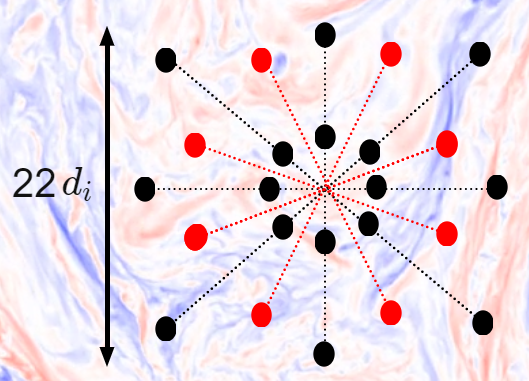
\includegraphics[width=1.\textwidth]{figures/chap8/spc_config_24.png}
                \caption[Configuration for 24 spacecraft]{One of the many configuration of
                spacecraft for 24 spacecraft. The inner black circles represent spacecraft at a
                distance of 2 $d_{\rm i}$ from the center whereas the outer ones are at 11 $d_{\rm
                i}$. The red dots are the spacecraft at 7 $d_{\rm i}$ from the center.}
                \label{fig:spc_conf}
            \end{center}
        \end{figure}

    \section{Methodology} \label{sec:method8}

        Simulation box size is $41.9\,d_{\rm i}$, and thus it takes the constellation roughly 10
        seconds to cross the whole box and each spacecraft makes 128 measurement in one flight. We
        use the synthetic time series data generated from the virtual spacecraft trajectory to train
        our GP model (see \Cref{sec:meth8} and \Cref{apdx:C}). If we have $N$ spacecraft in a given
        configuration and we have 128 observation along the $z$-axis. For one configuration we get
        $128 \times N$ data points for each component of the magnetic field to train our model. Once
        the training is complete, we feed in the coordinates of every point inside the disk of size
        28\,$d_{\rm i}$ (a few $d_{\rm i}$'s larger than the size of the constellation) for all the
        different planes, a total of 128 planes. This means for any number of spacecraft we must
        make predictions at $\sim 28 \times 28 \times 128$ points. This implies that greater number
        of spacecraft in any given configuration will give us better result since it will increase
        the amount of data used to train the model. However, as with any machine learning algorithm,
        there is a limit to how well trained a given model can be no matter the amount of input
        data. We discuss this in further detail in next section.

        Once we have the time series data, we trained the specified model on the observed data
        providing it one component at a time. Once the model is trained and the parameters of the
        model are learned based on the training set, we provide the model with all the locations in
        3-D space where we need to find the value of magnetic field. \Cref{apdx:C} gives the detail
        of implementation and also provide the code for the same.
    
    \section{Results} \label{sec:diss8}

        \Crefrange{fig:gpr_cas_bx}{fig:gpr_cas_bm} show one of the slice along xy-plane of the
        actual simulation data in Panel (\textbf{a}) (down sampled to 1\,$d_{\rm i}$ resolution) and
        the reconstructed field corresponding to different number of spacecraft employed (4 to 36,
        represented by the black dots) for observation (Panels \textbf{b} to \textbf{f}). For these
        figures, as discussed in \Cref{sec:meth8} reconstructed field were generated using kernel as
        defined in \Cref{eq:fin_ker_grd}. The configurations with 4 and 9 spacecraft poorly
        reproduce the original simulated field. Only when we have at least 16 spacecraft some
        structure is captured. Only for a constellation of 25 or more spacecraft does the
        reconstructed field closely resemble the original field structure. Though there is slight
        improvement in how well the original field is being captured when we  from 25 to 36
        spacecraft (as expected), whether this is worth additional expense of adding 11 more
        spacecraft need further investigation and a quantitative comparison.

        \begin{figure}
            \begin{center}
                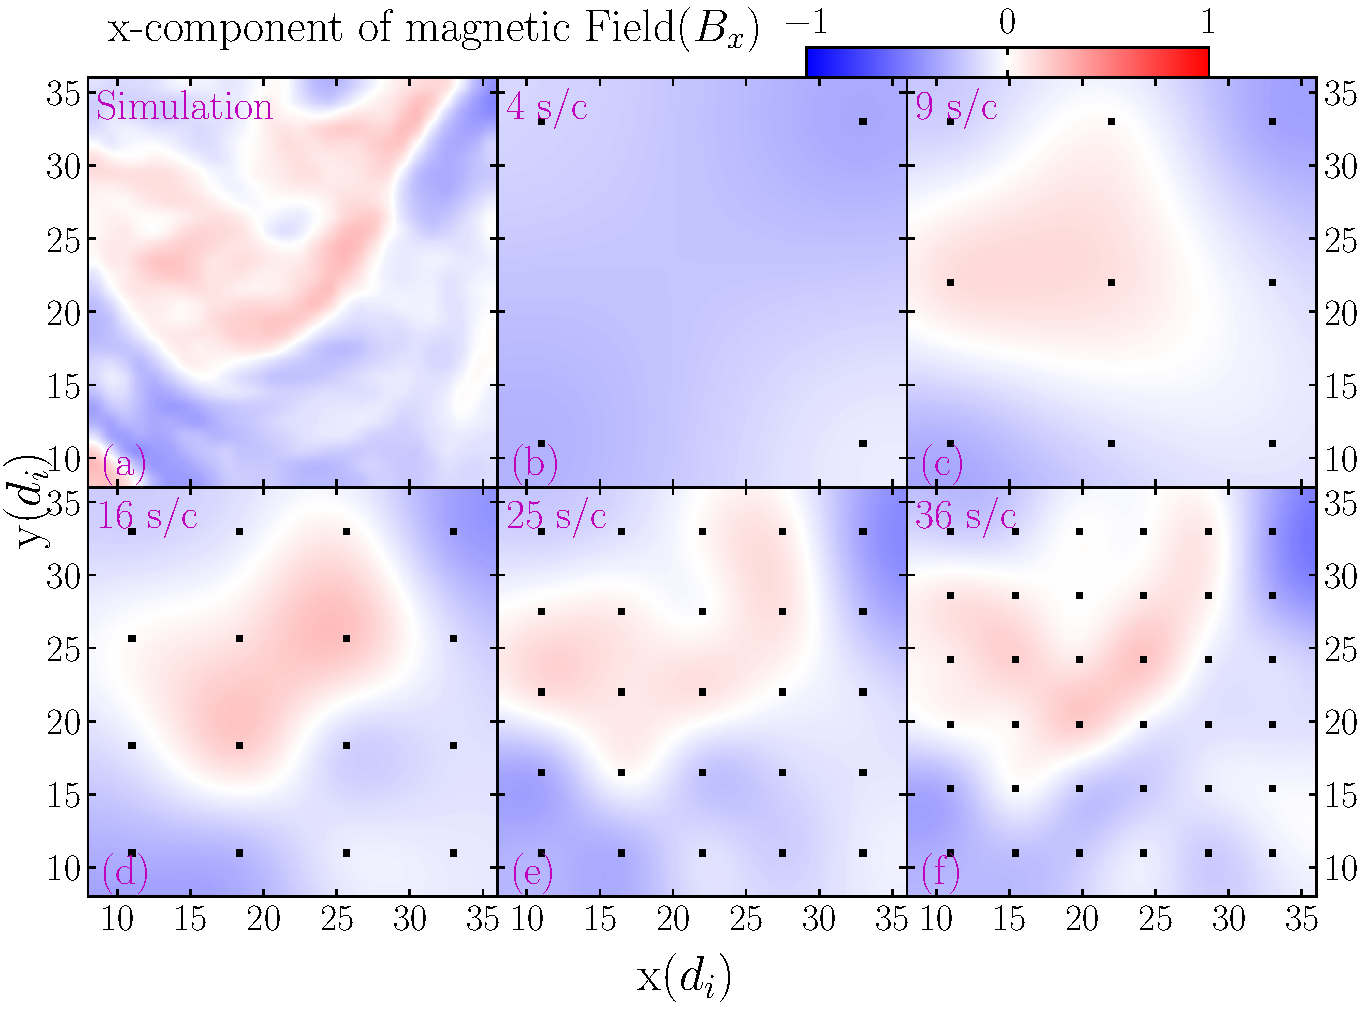
\includegraphics[width=0.85\textwidth, height=3.65in]{figures/chap8/all_spc_bx_4_9_16_25_36_001_cas1.pdf}
                \caption[Reconstructed field (x-component), linear configuration]{x-component of
                magnetic field from simulation (Panel \textbf{a}) and reconstructed field
                corresponding to different number of spacecraft (Panels \textbf{b} to \textbf{f})}
                \label{fig:gpr_cas_bx}
            \end{center}
        \end{figure}

        \begin{figure}
            \begin{center}
                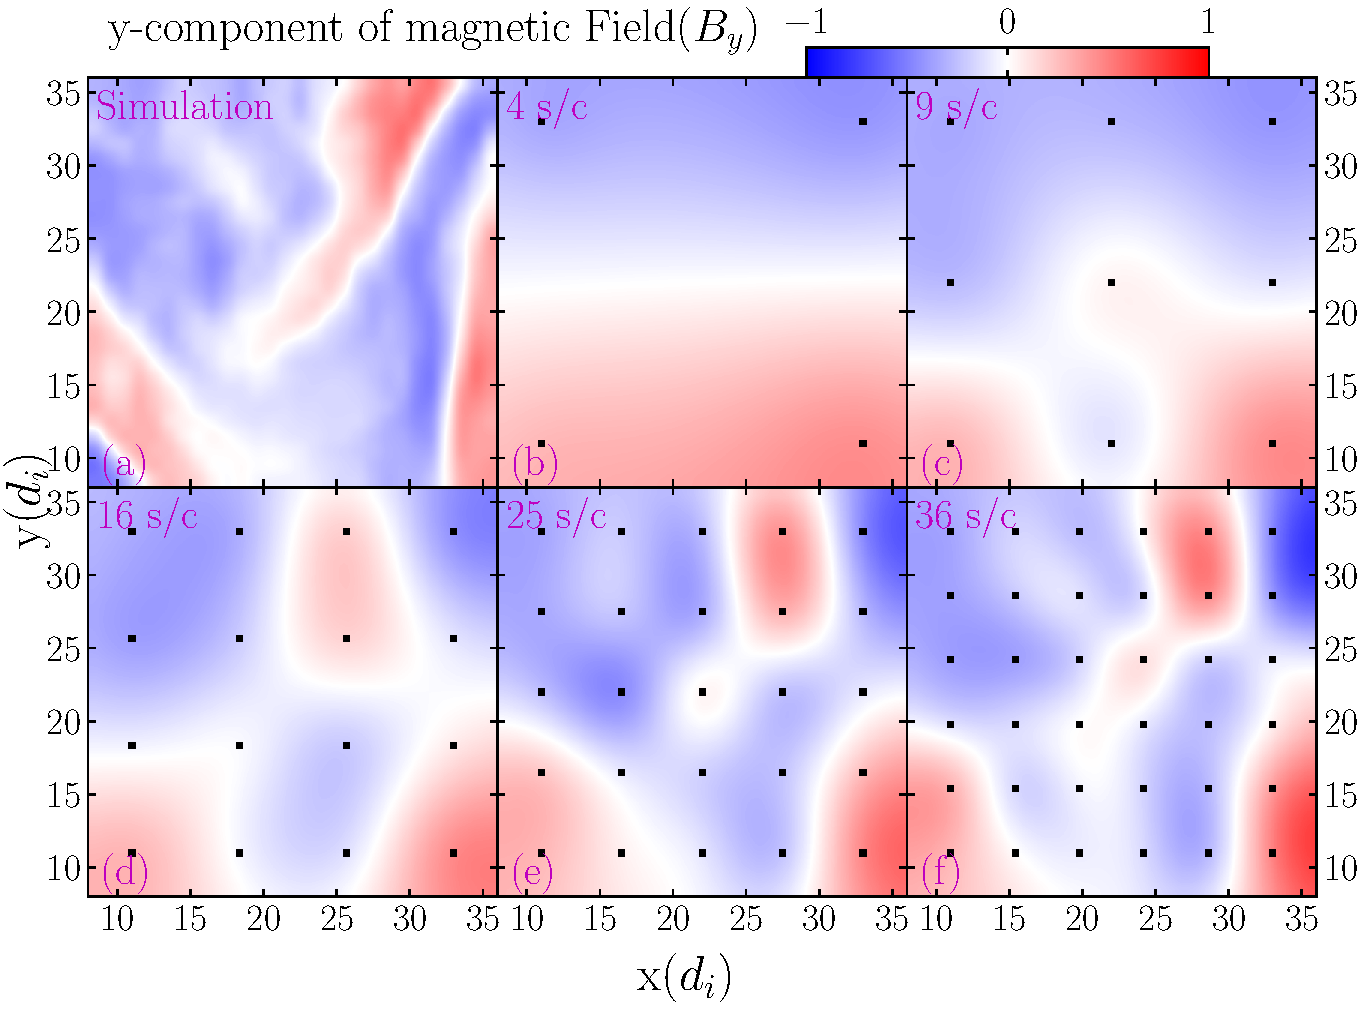
\includegraphics[width=0.85\textwidth, height=3.65in]{figures/chap8/all_spc_by_4_9_16_25_36_001_cas1.pdf}
                \caption[Reconstructed field (y-component), linear configuration]{y-component of
                magnetic field from simulation (Panel \textbf{a}) and reconstructed field
                corresponding to different number of spacecraft (Panels \textbf{b} to \textbf{f})}
                \label{fig:gpr_cas_by}
            \end{center}
        \end{figure}

        \begin{figure}
            \begin{center}
                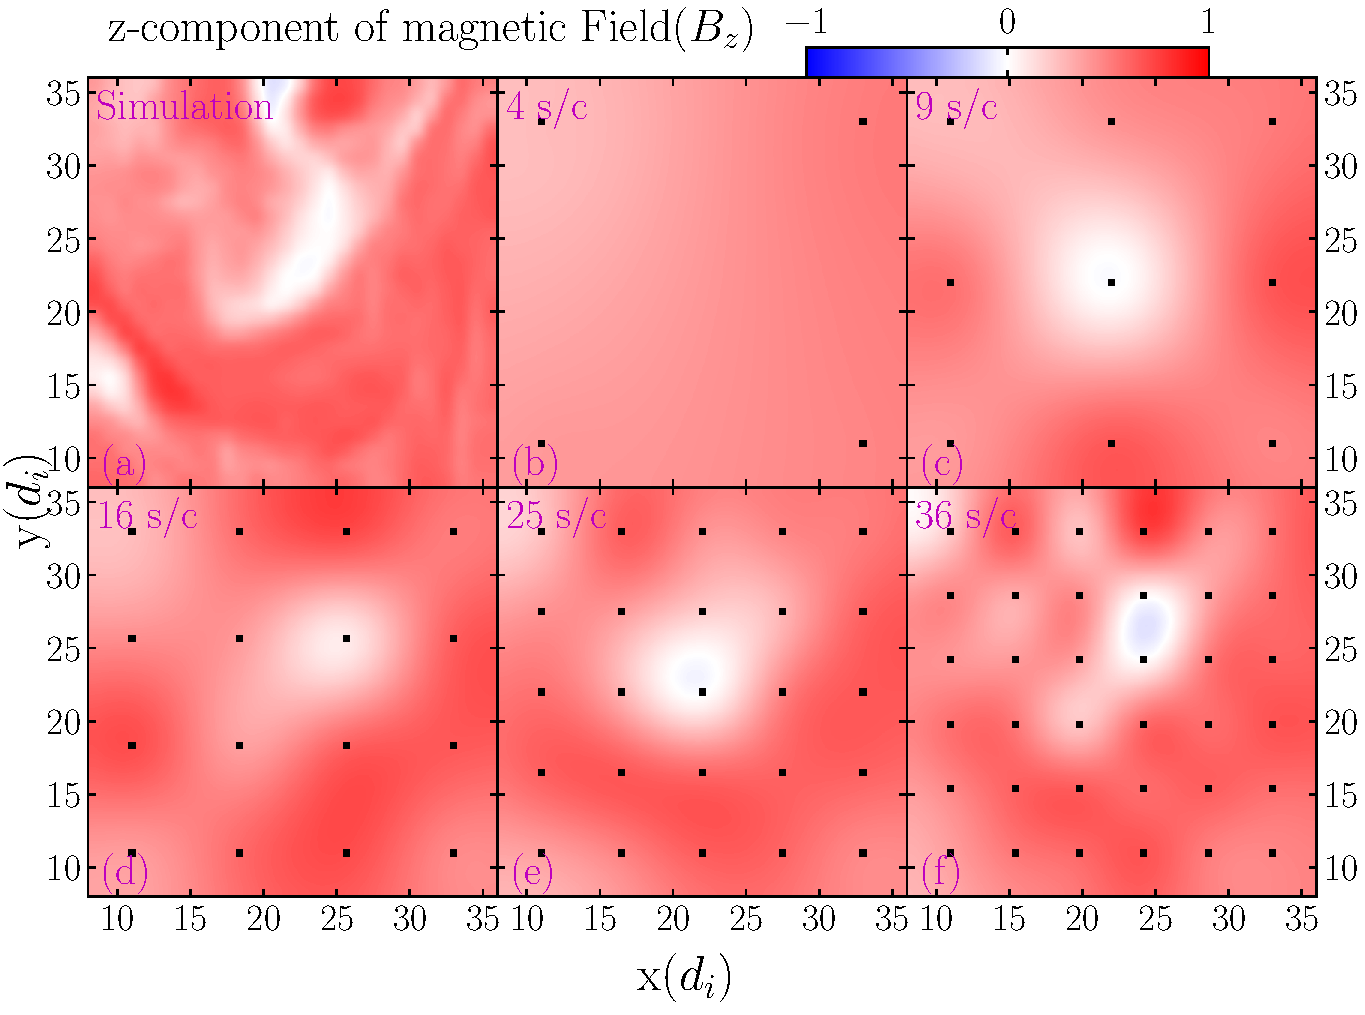
\includegraphics[width=0.85\textwidth, height=3.65in]{figures/chap8/all_spc_bz_4_9_16_25_36_001_cas1.pdf}
                \caption[Reconstructed field (z-component), linear configuration]{z-component of
                magnetic field from simulation (Panel \textbf{a}) and reconstructed field
                corresponding to different number of spacecraft (Panels \textbf{b} to \textbf{f})}
                \label{fig:gpr_cas_bz}
            \end{center}
        \end{figure}

        \begin{figure}
            \begin{center}
                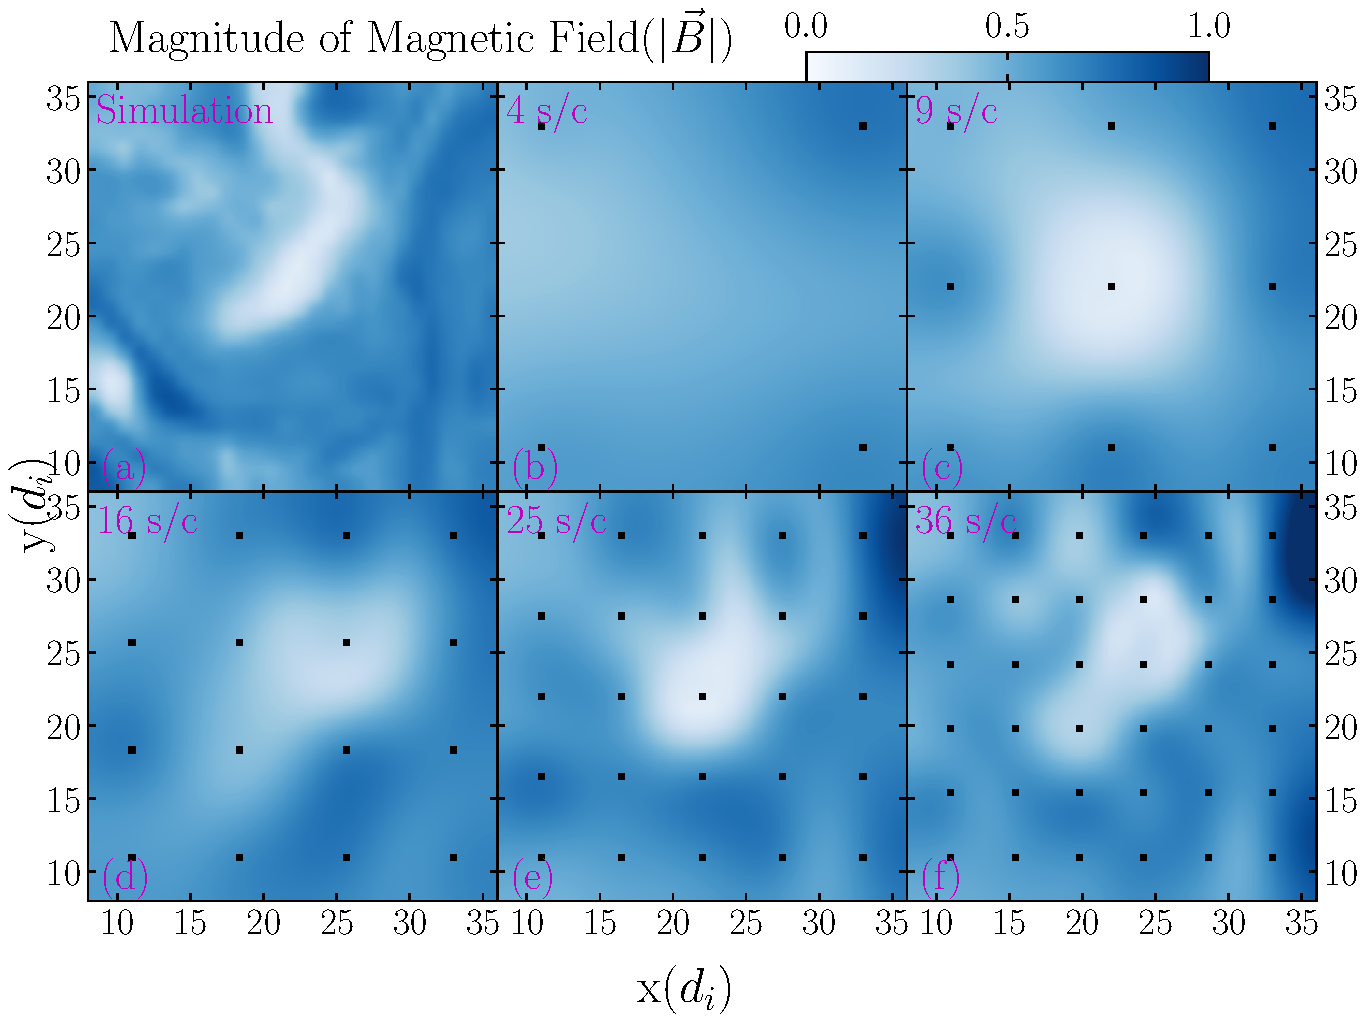
\includegraphics[width=0.85\textwidth, height=3.65in]{figures/chap8/all_spc_bm_4_9_16_25_36_001_cas1.pdf}
                \caption[Reconstructed field, linear configuration]{Magnitude of magnetic field from
                simulation (Panel \textbf{a}) and reconstructed field corresponding to different
                number of spacecraft (Panels \textbf{b} to \textbf{f})}
                \label{fig:gpr_cas_bm}
            \end{center}
        \end{figure}

        Results from circular configurations of spacecraft, for which the kernel in
        \Cref{eq:fin_ker_cir} was used, are shown in \Crefrange{fig:gpr_bx}{fig:gpr_bm}. As
        discussed for the previous figures, Panel (\textbf{a}) shows the original data, whereas
        Panels (\textbf{b}) to (\textbf{h}) show reconstructed field corresponding to different
        number of spacecraft. The spacecraft are distributed around a common center such that
        irrespective of the number of spacecraft employed, maximum distance between two spacecraft
        is always 22$\,d_{\rm i}$ so that they all cover equal volume of space in any given amount
        of time. As was the case for grid-like configuration, reconstructed fields do not capture
        any meaningful structure for 4 or 8 spacecraft. Some structure does show up for 16
        spacecraft however it is only when we employ 24 or more spacecraft that we get the structure
        of the field which looks similar to the original input (more on this later).

        For 24 spacecraft, we also randomized the position of each spacecraft, such that each
        spacecraft could be anywhere in a circle of radius 2$\,d_{\rm i}$ from its starting position
        (see Panel \textbf{g}). Reconstructed data, even for randomized position, continue to
        capture the actual structure of the original field. This observation considerably lessens
        the burden of having precisely defined orbits of each spacecraft. As long as individual
        spacecraft can communicate with each other regarding their relative position, reconstruction
        is not effected in a significant way.

        Given that we have a large number of spacecraft, at least 24, for this observation, a
        scenario might arise where one or more of them fail to function properly, either because of
        partial or full failure of instruments or for any other conceivable reason. We considered
        this scenario in the following way. We record the position of all spacecraft as shown in
        Panel (\textbf{g}) of \Crefrange{fig:gpr_bx}{fig:gpr_bm} and randomly remove two spacecraft,
        as shown in Panel (\textbf{h}) of the same figures. We then carry out GP on the modified
        data. Results from such reconstruction are shown in Panel (\textbf{h}) of each figure. As
        one can see, though the quality of reconstruction deteriorates a bit, compared to 24
        spacecraft (Panel \textbf{e}) it still manages to capture most of the structure present.
        These two observations (randomized location of spacecraft and random failing of 2 out of 24
        spacecraft) shows the robustness of algorithm.

        Based on the results we have shown so far, we thus conclude that if such an algorithm were
        to be applied, we will need at least 24 spacecraft in different configuration.
        \begin{figure}
            \begin{center}
                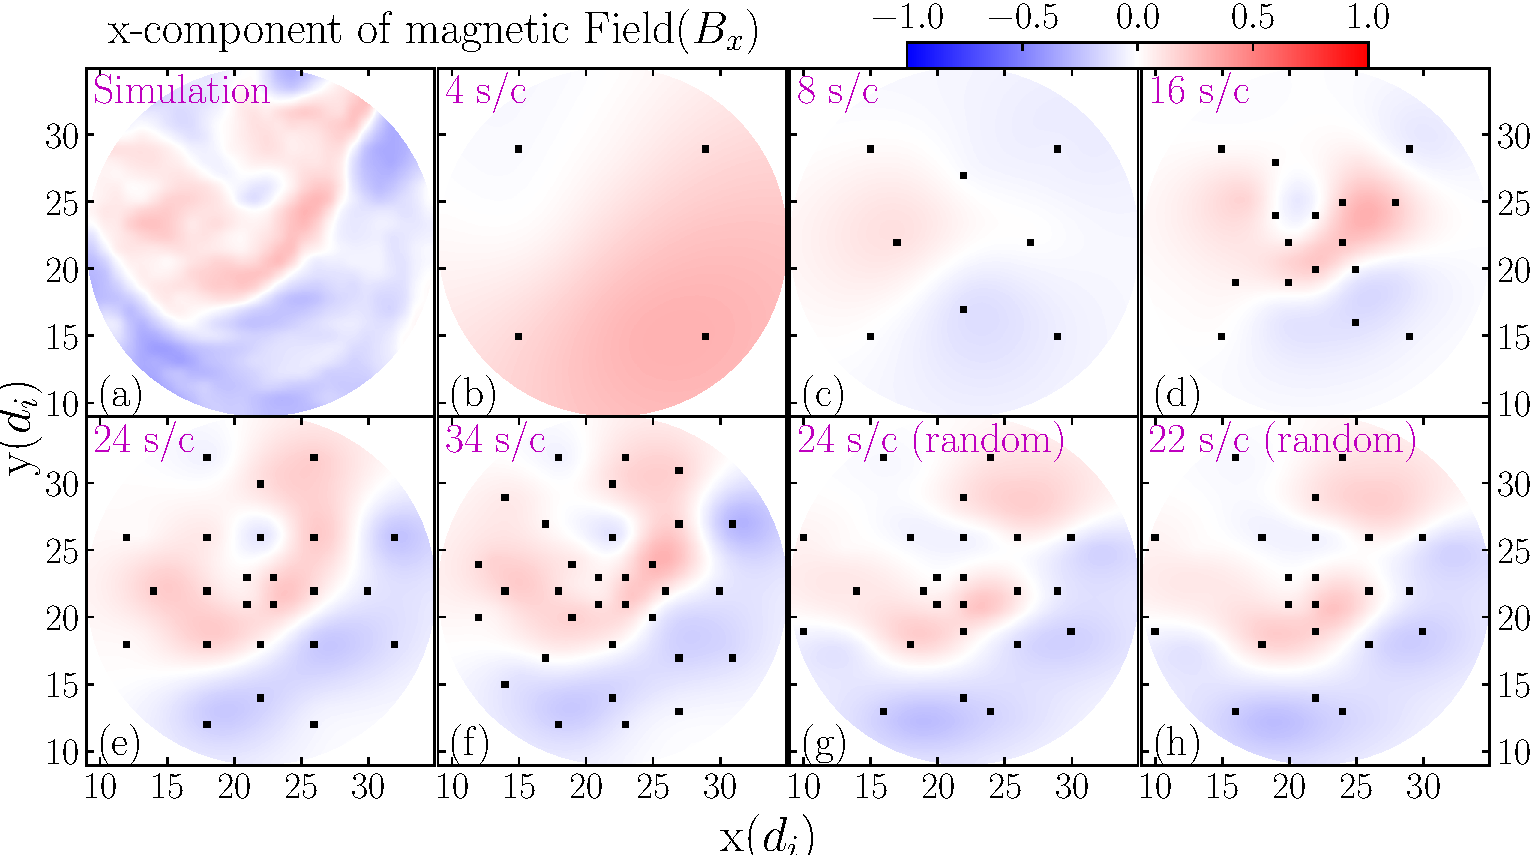
\includegraphics[width=0.85\textwidth]{figures/chap8/all_spc_bx_4_8_16_24_34_24_22_000.pdf}
                \caption[Reconstructed field (x-component), circular configuration]{x-component of the magnetic field from simulation (a) and various different number for circular configuration of spacecraft (b to h)}
                \label{fig:gpr_bx}
            \end{center}
        \end{figure}

        \begin{figure}
            \begin{center}
                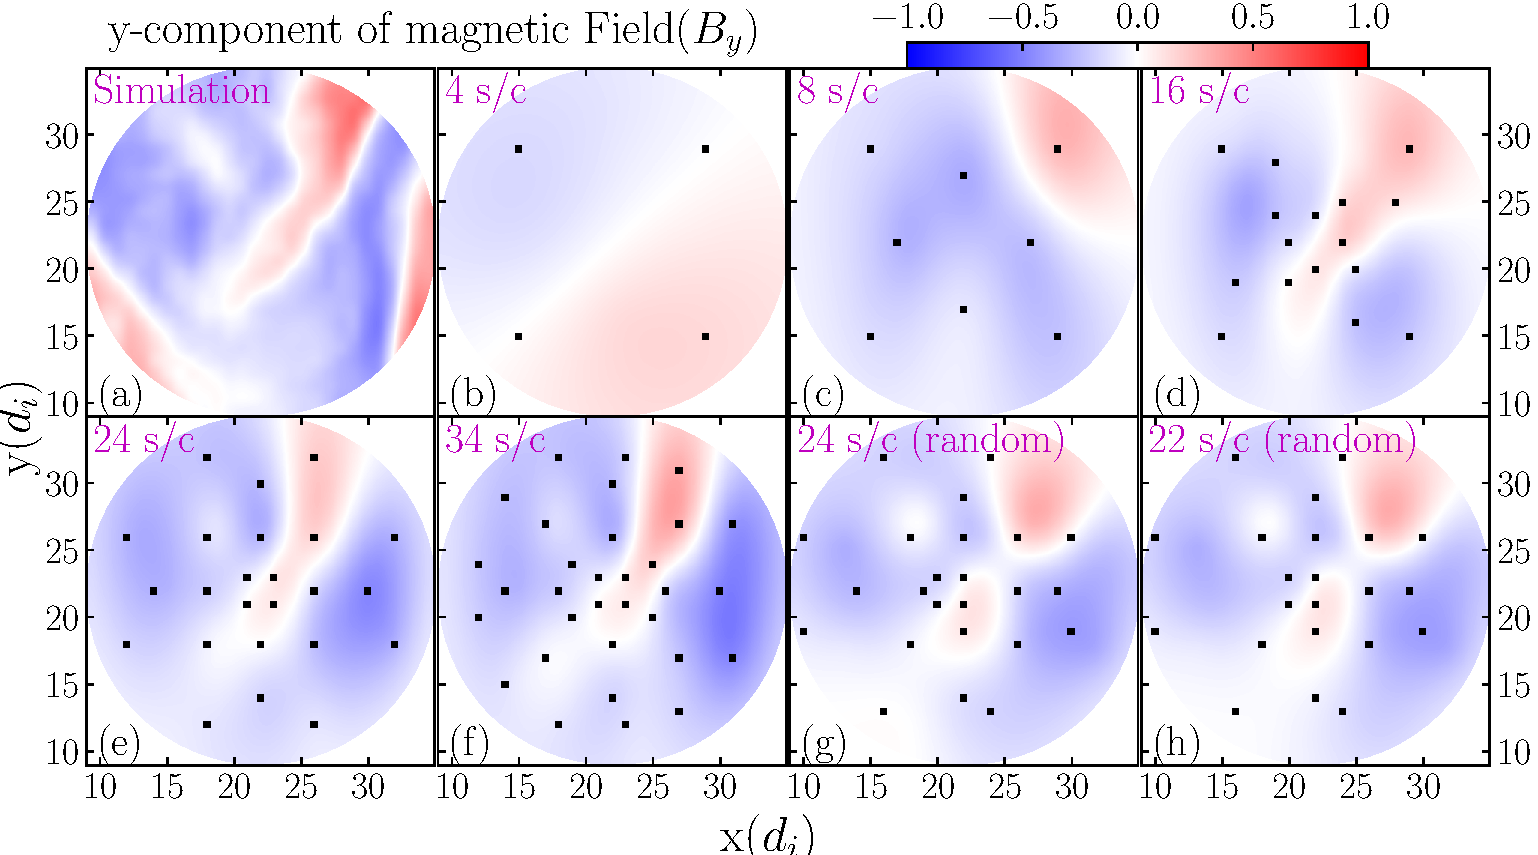
\includegraphics[width=0.85\textwidth]{figures/chap8/all_spc_by_4_8_16_24_34_24_22_000.pdf}
                \caption[Reconstructed field (y-component), circular configuration]{y-component of the magnetic field from simulation (a) and various different number for circular configuration of spacecraft (b to h)}
                \label{fig:gpr_by}
            \end{center}
        \end{figure}

        \begin{figure}
            \begin{center}
                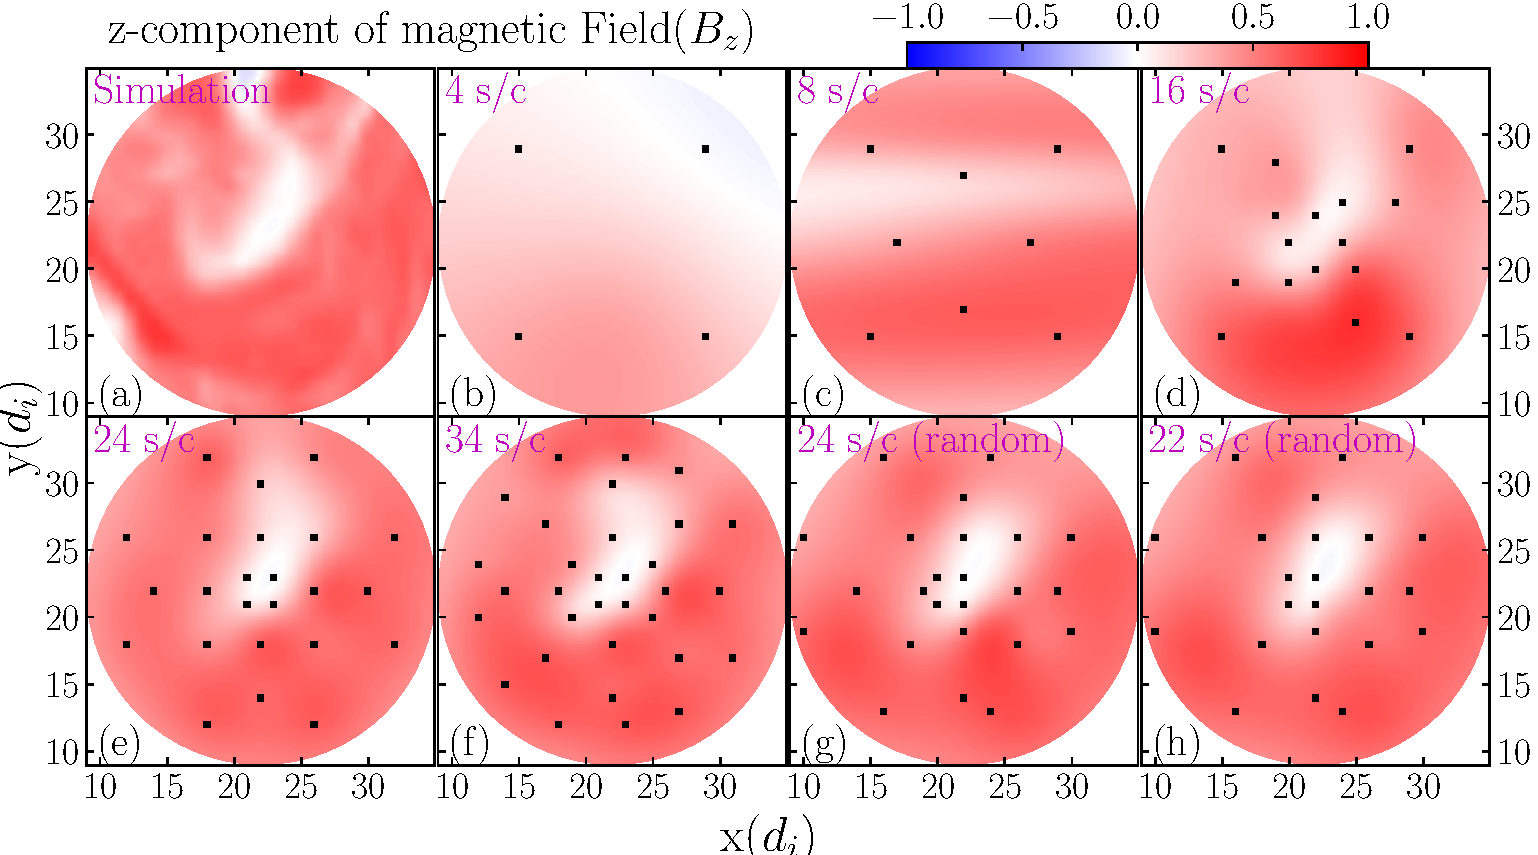
\includegraphics[width=0.85\textwidth]{figures/chap8/all_spc_bz_4_8_16_24_34_24_22_000.pdf}
                \caption[Reconstructed field (z-component), circular configuration]{z-component of the magnetic field from simulation (a) and various different number for circular configuration of spacecraft (b to h)}
                \label{fig:gpr_bz}
            \end{center}
        \end{figure}

        \begin{figure}
            \begin{center}
                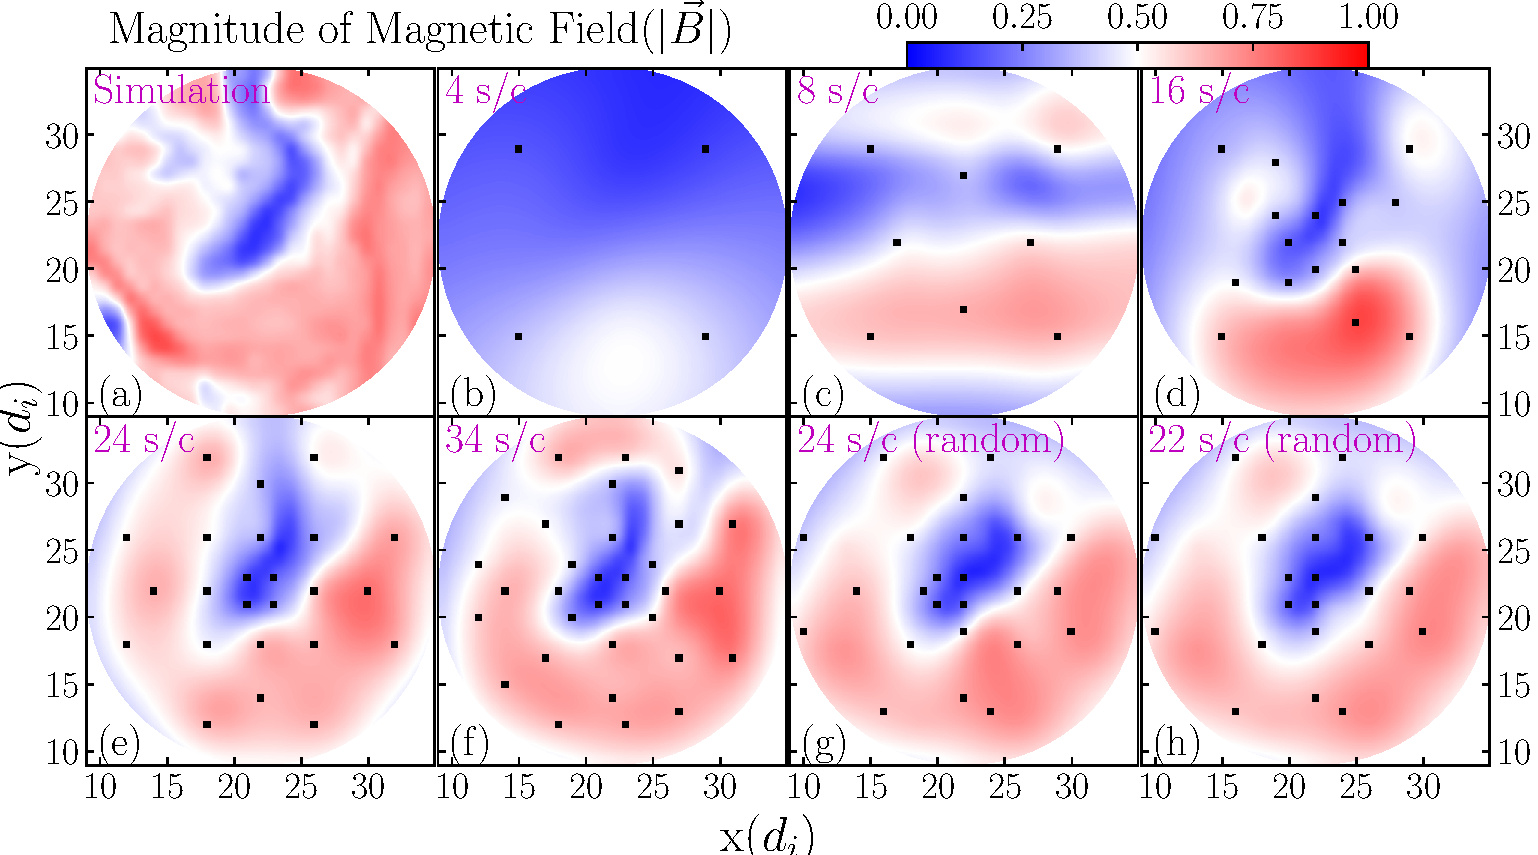
\includegraphics[width=0.85\textwidth]{figures/chap8/all_spc_bm_4_8_16_24_34_24_22_000.pdf}
                \caption[Reconstructed field, circular configuration]{Total magnetic field from simulation (a) and various different number for circular configuration of spacecraft (b to h)}
                \label{fig:gpr_bm}
            \end{center}
        \end{figure}
        
    \section{Discussions} \label{sec:conc8}

        The unknown nature of turbulence in the solar wind has given rise to competing theories to
        explain the structure and evolution of the interplanetary magnetic field and how energy is
        transferred from one scale to another. Measurements from a single spacecraft cannot
        differentiate between temporal and spatial fluctuations in the field and thus cannot
        conclusively support or reject any one of these theories. Measurements of the field's
        complete 3-D morphology and topology will enable us to understand the true nature of
        solar-wind turbulence. This study thus focused on determining the baseline number of
        spacecraft required to produce 3-D images of the IMF from in-situ magnetic field
        measurements.

        Using fully kinetic 3-D PIC simulation data, we demonstrated magnetic field topology
        reconstruction from synthetic time series in 3-D space using Gaussian Processes, a machine
        learning algorithm. Our results indicate that 24 spacecraft would be required for the
        satisfactory reconstruction of 3-D IMF structure. We also showed that precise control of
        spacecraft trajectory is not required for such a mission so long as the spacecraft positions
        are known. A baseline of 24 spacecraft even allows for unfavorable alignment of some
        spacecraft, though substantially fewer spacecraft (e.g., 16) fail to produce consistently
        adequate IMF reconstructions.

        Nevertheless, this study is still very much a work in progress and much needs to be done
        before we can reach a final version of the algorithm. As stated in \Cref{sec:meth8}, we
        applied GP to each component of the field individually, ignoring the other two components.
        In reality the magnetic field components are not fully independent since the magnetic field
        must be divergence-less.  In principle, a kernel could be implemented that would process all
        three components simultaneously and even enforce the requirement of a divergence-less field
        \citep[for a 2-D example of this, see][]{Narcowich2007,Wahlstroem2013}.  Alternatively a
        divergence cleaning algorithm could be applied after the GP algorithm has run. 
        
        We are also investigating alternative machine learning techniques. For example Deep GP
        \citep{Bui2016} can generate the best kernel for a given dataset rather than requiring the
        user to select one.

        More study is also required of how the arrangement of a given number of spacecraft affects
        the accuracy of magnetic reconstruction. A key component of this would be developing
        quantitative metrics for assessing reconstruction quality. A simple point by point
        comparison cannot take into account the benign distortion and blurring which arises because
        of reconstruction using a finite number of spacecraft. Instead, we are focusing on
        physically relevant parameters of magnetic structures: e.g., the connectivity of magnetic
        fields and the aspect ratios and orientations of regions of weak/strong magnetic field.